\documentclass[10pt,letterpaper]{article}
\usepackage[utf8]{inputenc}
\usepackage[english]{babel}
\usepackage{amsmath}
\usepackage{amsfonts}
\usepackage{amssymb}
\usepackage{graphicx}
\usepackage{listings}
\usepackage[pdftex]{hyperref}
\usepackage{multirow}


\hypersetup{colorlinks,%
	citecolor=black,%
	filecolor=black,%
	linkcolor=black,%
	urlcolor=blue}

\begin{document}

\begin{center}
	\textbf{Proyecto de Simulación}\\
	\textbf{Lógica Difusa}\\
	\textbf{Curso: 2019-2020}\\
\end{center}
		
\vspace{1.5cm}
		
Oscar Luis Hernández Solano \hspace{0.7cm}
\href{mailto:o.hernandez2@estudiantes.matcom.uh.cu}{o.hernandez2@estudiantes.matcom.uh.cu}

Grupo C411\\


\section{Introducción:}
Los Sistemas de Inferencia Difusa son una forma de representar conocimientos y datos inexactos en forma similar a como lo hace el pensamiento humano, este define una correspondencia no lineal entre una o varias variables de entrada y una variable de salida. Esto proporciona una base desde la cual pueden tomarse decisiones o definir patrones. El sistema de inferencia difusa implementado cuenta con Funciones de Pertenencia triangular y trapezoidal, los métodos de agregación de Mamdani y Larsen y los métodos de defusificación implementados son Centroide, Bisección y la Media de los Máximos.

\section{Aspectos generales:}

\begin{enumerate} 
\item \textbf{Funciones de Pertenencia:}
Una función de pertenencia de un conjunto difuso $A$ sobre un universo discurso $X$ es de la forma $\mu_{A}:X \rightarrow [0,1]$, donde a cada elemento de $X$ le corresponde un valor de pertenencia o grado de pertenencia, representa el grado en el que el elemento de $X$ pertenence al conjunto difuso $A$.\\
	
	\textbf{Función triangular:} Viene definida por un límite inferior $a$, un límite superior $b$ y un valor $m$ tal que $a < m < b$.
	\begin{align*}
		\mu_A (x) = \begin{cases}
		0, & x \leq a \\\\
		\dfrac{x - a}{m - a}, & a < x \leq m \\\\
		\dfrac{b - x}{b - m}, & m < x < b \\\\
		0, & x \ge b
		\end{cases}
	\end{align*}\\
	
	\textbf{Función trapezoidal:} Viene definida por un límite inferior $a$, un límite superior $d$, un límite de soporte inferior $b$ y un límite de soporte superior $c$, tal que $a < b < c < d$.
	\begin{align*}
		\mu_A (x) = \begin{cases}
		0, & x < a \\\\
		\dfrac{x - a}{b - a}, & a \leq x \leq b \\\\
		1, & b \leq x \leq c \\\\
		\dfrac{d - x}{d - c}, & c \leq x \leq d \\\\
		0, & x > d
		\end{cases}
	\end{align*}
	
\item \textbf{Métodos de Agregación:}
El sistema emplea los m\'etodos de Mamdani y Larsen para determinar una agregaci\'on, se determinan los valores de los $\alpha_i$ dependiendo del tipo de entrada y luego se determina la funci\'on de pertenencia para la agregaci\'on $C'$:

	\begin{enumerate}
		\item[] \textbf{Mamdani}: $\mu_{C'} (z) = \bigvee_{i=1}^{n} \left[ \alpha_i  \wedge \mu_{C_i} (z) \right]$ 
		
		\item[] \textbf{Larsen}: $\mu_{C'} (z) = \bigvee_{i=1}^{n} \left[ \alpha_i \cdot \mu_{C_i} (z) \right]$\\
	\end{enumerate}


\item \textbf{Métodos de Desfusificación:}
El proceso de desfusificación permite asociar a un conjunto difuso un valor numérico y se lleva a cabo para calcular el valor de salida de los modelos difusos.

	\begin{enumerate}
		\item[] \textbf{Centroide:} Asocia el centro del área formada por el número difuso. Matemáticamente se expresa de la siguiente forma:
		\begin{align*}
		C = \frac{ \int_{S} x\mu (x) \;dx }{ \int_{S} \mu (x) \;dx }  
		\end{align*}
		donde $\mu(x)$ es la función de pertenencia del conjunto de salida, cuya variable es $x$ y $S$ es el dominio o rango de integración.\\
		
		\item[] \textbf{Bisectriz:} Es un método que trata de encontrar el valor del elemento del universo que separa el área de la función de pertenencia del conjunto difuso en dos mitades con la misma área.\\
		
		\item[] \textbf{Máximo Central:} Máximo Central o media de los máximos da como salida el valor medio de todos aquellos que generan el valor más alto de la función de pertenencia.
	\end{enumerate}

\end{enumerate}


\section{Descripción del Sistema:}

\begin{enumerate}
	\item[] $FuzzySet$ define el concepto de conjunto difuso esta compuesta por su función de pertenecia y cuenta además con un conjunto de funcionalidades aplicables a conjuntos difusos como son la Unión, Intersección, Complemento y Corte.
	
	\item[] $FuzzyVariable$ define el concepto de variable difusa, la caracterizan su universo discurso y el set de conjuntos difusos que la componen.
	
	\item[] $FuzzySystem$ define el concepto del sistema difuso y recibe un conjunto de variables de entrada, un conjunto de variables de salida y un conjunto de reglas. Aquí se evalúan las reglas según los valores de entrada usando el método de agregación deseado y finalmente se aplican los métodos de desfusificación a la agregación resultante. Cuenta además con una funcionalidad para representar el sistema de inferencia difusa gráficamente.
\end{enumerate}


\section{Problema:}
El seguro del automóvil es un contrato de seguro que cubre los riesgos creados por la conducción de automóviles en caso de causar un accidente. Existe una modalidad básica, cuya contratación es obligatoria por los propietarios de todo vehículo, denominada por ello seguro obligatorio del automóvil que cubre la responsabilidad civil del propietario y del conductor del vehículo. Una compañía de seguros, necesita evaluar el riesgo financiero de sus clientes que requieren póliza de seguros contra accidentes automovilísticos. Para evaluar el riesgo financiero se toma en cuenta la edad del asegurado y su porcentaje de manejo durante el año.

\begin{enumerate}
	\item \textbf{Variables:}
		\begin{enumerate}
			\item[] \textbf{Edad:}
				\begin{enumerate}
					\item[] $U = [18, 70]$
					\item[] Jóven: $Trapezoidal(18, 18, 25, 30)$
					\item[] Adulto: $Triangular(20, 35, 50)$
					\item[] Mayor: $Trapezoidal(40, 60, 70, 70)$
				\end{enumerate}
			
			\item[]	\textbf{Porciento de Manejo:}
				\begin{enumerate}
					\item[] $U = [0, 100]$
					\item[] Bajo: $Trapezoidal(0, 0, 10, 20)$
					\item[] Medio: $Triangular(10, 40, 60)$
					\item[] Alto: $Trapezoidal(50, 70, 100, 100)$
				\end{enumerate}
			
			\item[] \textbf{Riesgo financiero:}
				\begin{enumerate}
					\item[] $U = [0, 100]$
					\item[] Bajo: $Trapezoidal(0, 0, 10, 20)$
					\item[] Medio: $Triangular(10, 30, 45)$
					\item[] Alto: $Trapezoidal(50, 70, 100, 100)$
				\end{enumerate}
		\end{enumerate}

	\item \textbf{Reglas:}\\

		\begin{tabular}{ |l|r|r|r| }
			\hline
			& Edad - Jóven & Edad - Adulto & Edad - Mayor\\
			\hline
			 Manejo - Bajo & Riesgo - Medio & Riesgo - Bajo & Riesgo - Medio\\
			\hline
			Manejo - Medio & Riesgo - Alto & Riesgo - Medio & Riesgo - Alto\\
			\hline
			Manejo - Alto & Riesgo - Alto & Riesgo - Alto & Riesgo - Alto\\
			\hline
		\end{tabular}


\section{Resultados:}
Una vez definidas las variables y el conjunto de reglas, pasamos a resolver el sistema para ello utilizamos dos entradas $(25, 50), (52, 63)$ y probamos los resultados utiliando los dos métodos de agregación y los tres métodos de desfusificación. La salida del programa será la siguiente:

		
\begin{verbatim}
	sample_0
	
	{'Edad': 25, 'Manejo': 50}
	Método: Mamdani
	Centroide: 61.01798855
	Bisectriz: 62.62626263
	Media de los Máximos: 74.24242424
	
	Método: Larsen
	Centroide: 65.73982862
	Bisectriz: 68.68686869
	Media de los Máximos: 77.77777778
	
	sample_1
	
	{'Edad': 52, 'Manejo': 63}
	Método: Mamdani
	Centroide: 72.44105597
	Bisectriz: 72.72727273
	Media de los Máximos: 74.74747475
	
	Método: Larsen
	Centroide: 73.82422233
	Bisectriz: 73.73737374
	Media de los Máximos: 77.77777778
\end{verbatim}

\end{enumerate}

\vspace{1cm}

Al analizar los resultados de las pruebas realizadas podemos observar que ambos métodos Mamdani y Larsen se comportan de manera similar produciendo resultados con muy poca diferencia entre sí, de la misma manera los métodos de desfusificación Centroide y Bisectriz arrojan resultados bien cercanos e interesante como efectivamente reflejan en cierta medida un mayor riesgo financiero por parte del asegurado del ejemplo 2 que constituye una persona mayor y con más porcentaje de conducción anual que el asegurado del ejemplo 1.


\begin{figure}
	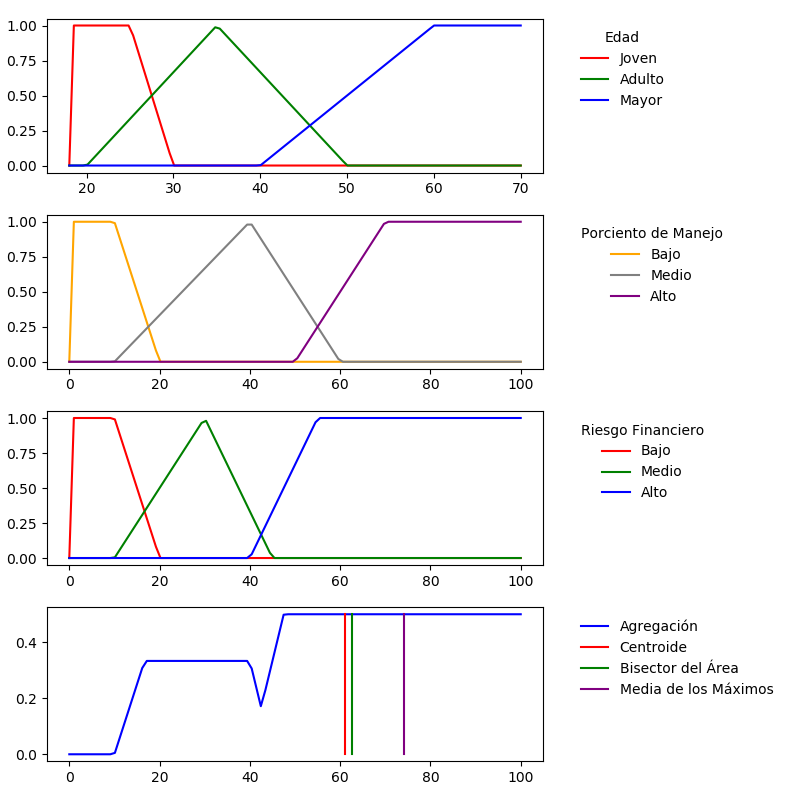
\includegraphics[width=\linewidth]{Figure_1.png}
	\caption{Ejemplo número 1 usando el método de agregación de Mamdani}
\end{figure}
 
 
		
\end{document}
	
	

	
	